\section{Vorgehen}
In diesem Kapitel wird das Vorgehen beschrieben, wie die Arbeit geplant und erledigt wurde.

\subsection{Arbeitsmethodik}
Um die Übersicht nicht zu verlieren, wurde beschlossen, nach Kanban zu arbeiten. Da eigens für die Arbeit ein Repository auf \emph{github.com}\footnote{\href{https://github.com/bfh-semesterarbeit/spot-geoprocessing/projects/1}{Projekt auf github.com}} angelegt wurde, konnte auch gleich ein Kanban erstellt werden.
\textbf{TODO: Theorie über Kanban - evtl. mit Fachbegriffen verhängen}

\begin{figure}[H]
	\centering
	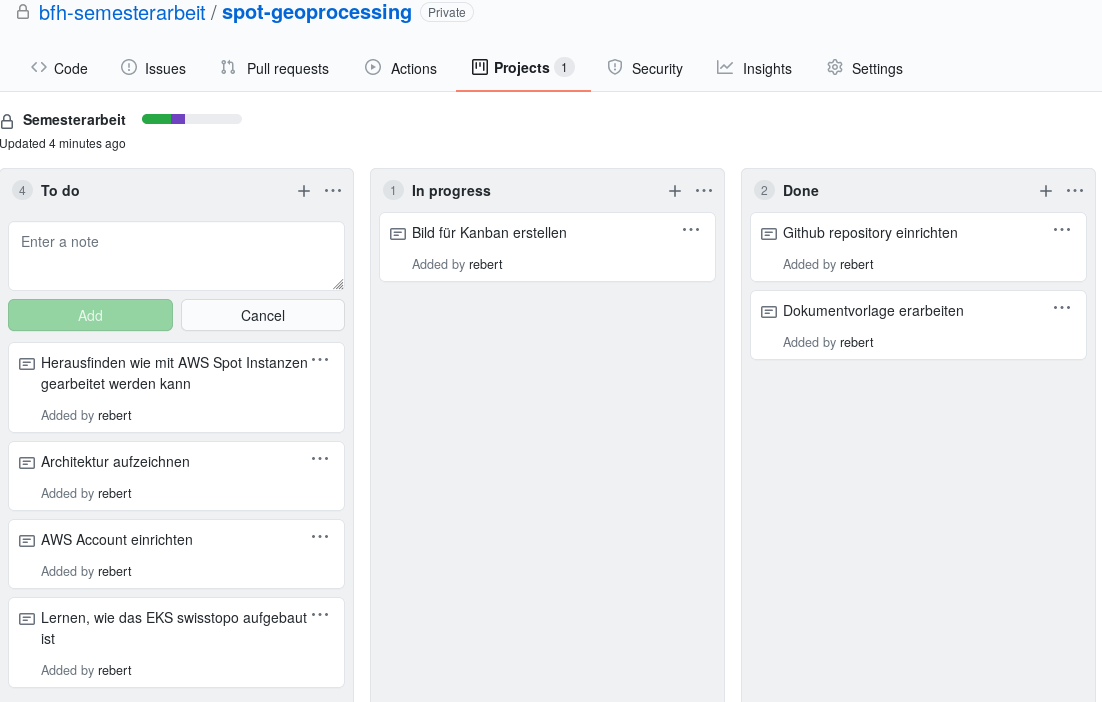
\includegraphics[width=.95\textwidth]{kanban}
	\caption{Klassisches Kanban auf \emph{github.com}}
	\label{fig:Klassisches Kanban}
\end{figure}

\subsection{Arbeitsweise}
Der Experte \prof \space begleitet die Arbeit seit unserem ersten Treffen, das vom 14. Juli 2020. Wir sind so verblieben.... , dass wir uns dann und wann wieder treffen. Die Arbeit, wie im Projektplan und in den Kanban Tickets definiert abgearbeitet wird... bei Fragen ...

\subsection{Projektplan}
\href{https://docs.google.com/spreadsheets/d/1zKTZgt4BW736G0xRfU9o3vWYwAJj-8nzFvGsPR7yJ_0/edit?usp=sharing}{Projektplan}\footnote{\href{https://docs.google.com/spreadsheets/d/1zKTZgt4BW736G0xRfU9o3vWYwAJj-8nzFvGsPR7yJ_0/edit?usp=sharing/edit?usp=sharing}{URL Google Spreadsheet}}

\section{Vorarbeiten}
\subsection{AWS Account}
\begin{itemize}
	\item Fit werden mit AWS
\end{itemize}

\subsection{AWS Spot Instances}
\begin{itemize}
	\item Herausfinden wie mit AWS Spot Instanzen gearbeitet werden kann
\end{itemize}
\begin{figure}[H]
	\centering
	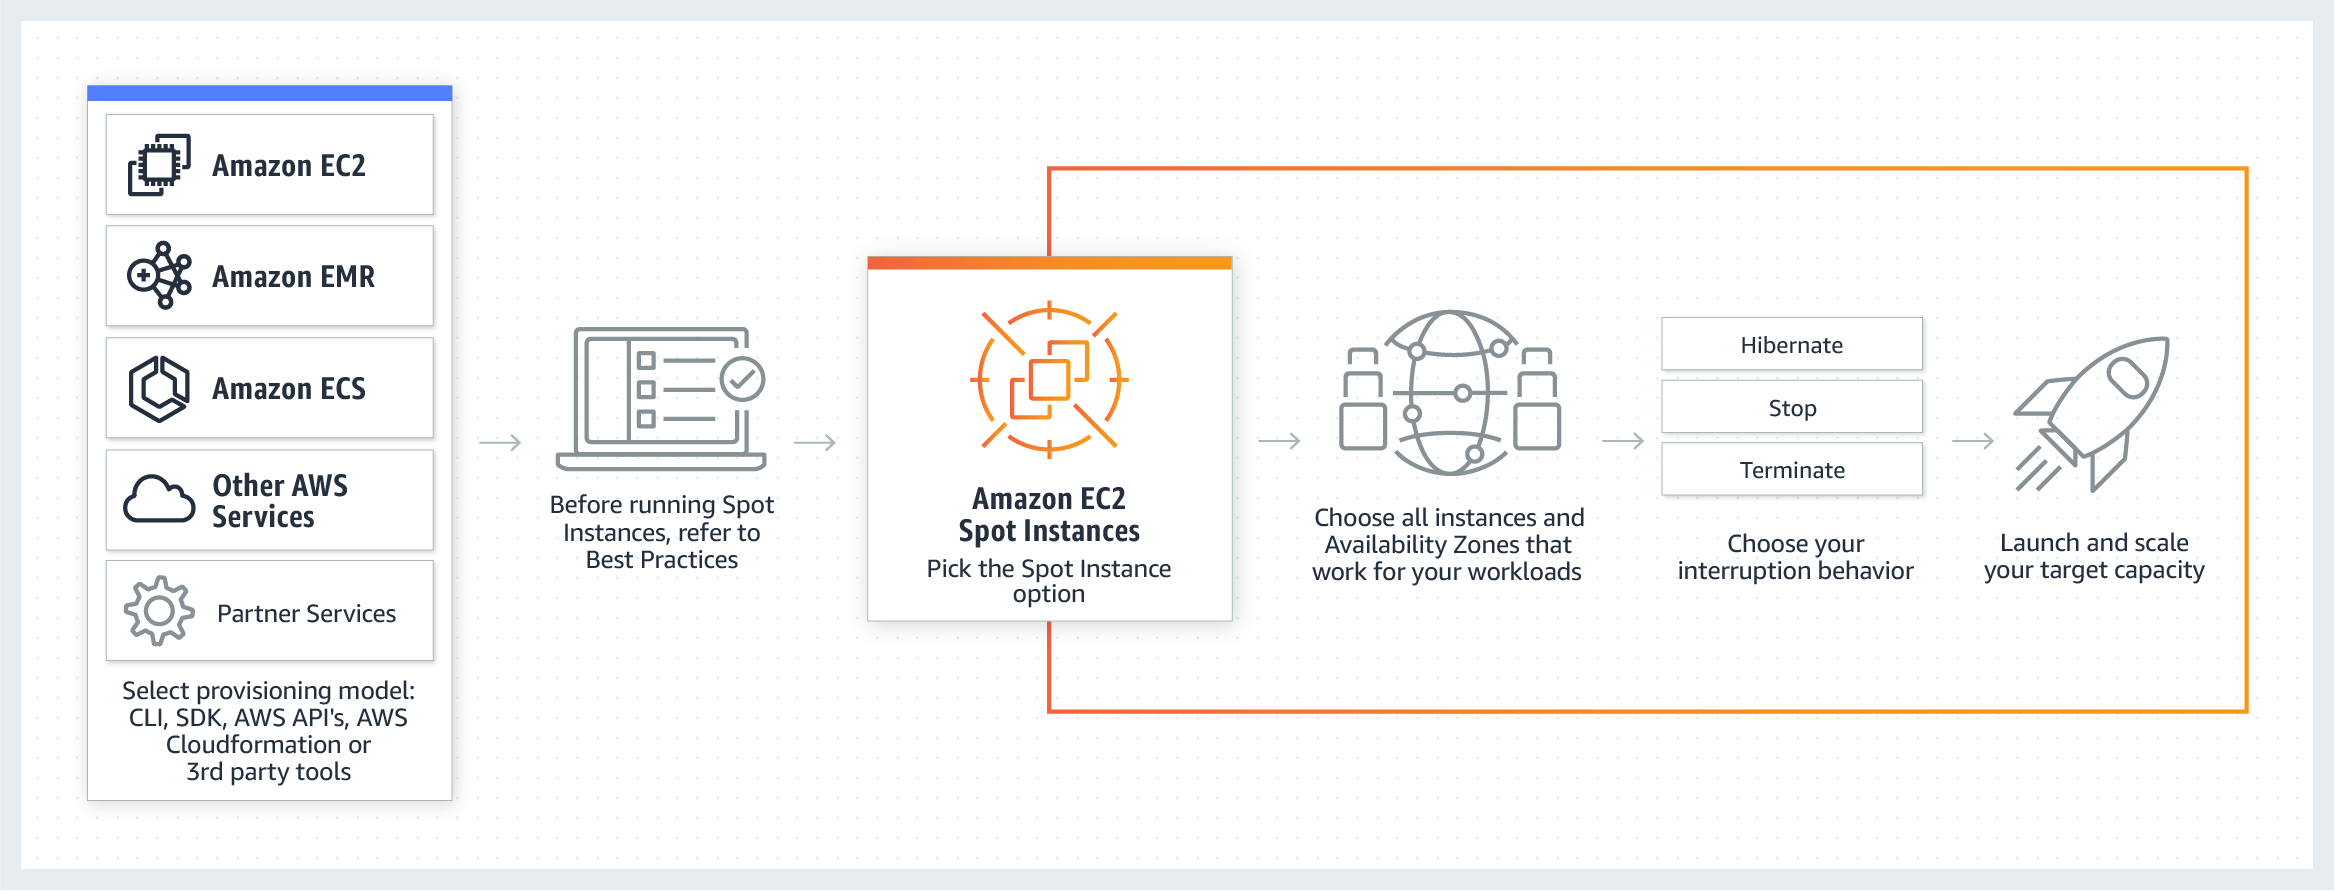
\includegraphics[width=.6\textwidth]{spot}
	\caption{AWS Architektur Spot\cite{AmazonAWSSpot:1}}
	\label{fig:AWS Architektur Spot}
\end{figure}

\subsection{Kubernetes testing}
\begin{itemize}
	\item Anfangs mit Minicube
	\item Eigenem AWS account
\end{itemize}
